\let\negmedspace\undefined
\let\negthickspace\undefined
\documentclass[journal,12pt,twocolumn]{IEEEtran}
%\documentclass[conference]{IEEEtran}
%\IEEEoverridecommandlockouts
% The preceding line is only needed to identify funding in the first footnote. If that is unneeded, please comment it out.
\usepackage{cite}
\usepackage{amsmath,amssymb,amsfonts,amsthm}
\usepackage{algorithmic}
\usepackage{graphicx}
\usepackage{textcomp}
\usepackage{xcolor}
\usepackage{txfonts}
\usepackage{listings}
\usepackage{enumitem}
\usepackage{caption}
\usepackage{mathtools}
\usepackage{gensymb}
\usepackage[breaklinks=true]{hyperref}
\usepackage{tkz-euclide} % loads  TikZ and tkz-base
\usepackage{listings}
%
%\usepackage{setspace}
%\usepackage{gensymb}
%\doublespacing
%\singlespacing

%\usepackage{graphicx}
%\usepackage{amssymb}
%\usepackage{relsize}
%\usepackage[cmex10]{amsmath}
%\usepackage{amsthm}
%\interdisplaylinepenalty=2500
%\savesymbol{iint}
%\usepackage{txfonts}
%\restoresymbol{TXF}{iint}
%\usepackage{wasysym}
%\usepackage{amsthm}
%\usepackage{iithtlc}
%\usepackage{mathrsfs}
%\usepackage{txfonts}
%\usepackage{stfloats}
%\usepackage{bm}
%\usepackage{cite}
%\usepackage{cases}
%\usepackage{subfig}
%\usepackage{xtab}
%\usepackage{longtable}
%\usepackage{multirow}
%\usepackage{algorithm}
%\usepackage{algpseudocode}
%\usepackage{enumitem}
%\usepackage{mathtools}
%\usepackage{tikz}
%\usepackage{circuitikz}
%\usepackage{verbatim}
%\usepackage{tfrupee}
%\usepackage{stmaryrd}
%\usetkzobj{all}
%    \usepackage{color}                                            %%
%    \usepackage{array}                                            %%
%    \usepackage{longtable}                                        %%
%    \usepackage{calc}                                             %%
%    \usepackage{multirow}                                         %%
%    \usepackage{hhline}                                           %%
%    \usepackage{ifthen}                                           %%
  %optionally (for landscape tables embedded in another document): %%
%    \usepackage{lscape}     
%\usepackage{multicol}
%\usepackage{chngcntr}
%\usepackage{enumerate}

%\usepackage{wasysym}
%\newcounter{MYtempeqncnt}
\DeclareMathOperator*{\Res}{Res}
%\renewcommand{\baselinestretch}{2}
\renewcommand\thesection{\arabic{section}}
\renewcommand\thesubsection{\thesection.\arabic{subsection}}
\renewcommand\thesubsubsection{\thesubsection.\arabic{subsubsection}}

\renewcommand\thesectiondis{\arabic{section}}
\renewcommand\thesubsectiondis{\thesectiondis.\arabic{subsection}}
\renewcommand\thesubsubsectiondis{\thesubsectiondis.\arabic{subsubsection}}

% correct bad hyphenation here
\hyphenation{op-tical net-works semi-conduc-tor}
\def\inputGnumericTable{}                                 %%

\lstset{
%language=C,
frame=single, 
breaklines=true,
columns=fullflexible
}
%\lstset{
%language=tex,
%frame=single, 
%breaklines=true
%}

\begin{document}
%


\newtheorem{theorem}{Theorem}[section]
\newtheorem{problem}{Problem}
\newtheorem{proposition}{Proposition}[section]
\newtheorem{lemma}{Lemma}[section]
\newtheorem{corollary}[theorem]{Corollary}
\newtheorem{example}{Example}[section]
\newtheorem{definition}[problem]{Definition}
%\newtheorem{thm}{Theorem}[section] 
%\newtheorem{defn}[thm]{Definition}
%\newtheorem{algorithm}{Algorithm}[section]
%\newtheorem{cor}{Corollary}
\newcommand{\BEQA}{\begin{eqnarray}}
\newcommand{\EEQA}{\end{eqnarray}}
\newcommand{\define}{\stackrel{\triangle}{=}}

\bibliographystyle{IEEEtran}
%\bibliographystyle{ieeetr}


\providecommand{\mbf}{\mathbf}
\providecommand{\pr}[1]{\ensuremath{\Pr\left(#1\right)}}
\providecommand{\qfunc}[1]{\ensuremath{Q\left(#1\right)}}
\providecommand{\sbrak}[1]{\ensuremath{{}\left[#1\right]}}
\providecommand{\lsbrak}[1]{\ensuremath{{}\left[#1\right.}}
\providecommand{\rsbrak}[1]{\ensuremath{{}\left.#1\right]}}
\providecommand{\brak}[1]{\ensuremath{\left(#1\right)}}
\providecommand{\lbrak}[1]{\ensuremath{\left(#1\right.}}
\providecommand{\rbrak}[1]{\ensuremath{\left.#1\right)}}
\providecommand{\cbrak}[1]{\ensuremath{\left\{#1\right\}}}
\providecommand{\lcbrak}[1]{\ensuremath{\left\{#1\right.}}
\providecommand{\rcbrak}[1]{\ensuremath{\left.#1\right\}}}
\theoremstyle{remark}
\newtheorem{rem}{Remark}
\newcommand{\sgn}{\mathop{\mathrm{sgn}}}
\providecommand{\abs}[1]{\left\vert#1\right\vert}
\providecommand{\res}[1]{\Res\displaylimits_{#1}} 
\providecommand{\norm}[1]{\left\lVert#1\right\rVert}
%\providecommand{\norm}[1]{\lVert#1\rVert}
\providecommand{\mtx}[1]{\mathbf{#1}}
\providecommand{\mean}[1]{E\left[ #1 \right]}
\providecommand{\fourier}{\overset{\mathcal{F}}{ \rightleftharpoons}}
%\providecommand{\hilbert}{\overset{\mathcal{H}}{ \rightleftharpoons}}
\providecommand{\system}{\overset{\mathcal{H}}{ \longleftrightarrow}}
 %\newcommand{\solution}[2]{\textbf{Solution:}{#1}}
\newcommand{\solution}{\noindent \textbf{Solution: }}
\newcommand{\cosec}{\,\text{cosec}\,}
\providecommand{\dec}[2]{\ensuremath{\overset{#1}{\underset{#2}{\gtrless}}}}
\newcommand{\myvec}[1]{\ensuremath{\begin{pmatrix}#1\end{pmatrix}}}
\newcommand{\mydet}[1]{\ensuremath{\begin{vmatrix}#1\end{vmatrix}}}
%\numberwithin{equation}{section}
%\numberwithin{equation}{subsection}
%\numberwithin{problem}{section}
%\numberwithin{definition}{section}
%\makeatletter
%\@addtoreset{figure}{problem}
%\makeatother



\title{Project Report - Random Audio Playlist Player}
\author{AI22BTECH11022, RUVVA SURAJ KUMAR}

\begin{document}

\maketitle

\section{Abstract}

This lab report presents a program that plays audio files randomly from a given playlist directory using the Pygame library in Python. The program allows the user to control the playback, next songs,repeart the playlist and quit the playlist. The playlist is shuffled using the NumPy library to provide a random order of songs.

\section{Introduction}

The goal of this project is to create a random audio playlist player that provides a seamless and interactive experience for the user. The program utilizes Pygame, a popular multimedia library in Python, to handle audio playback. The playlist directory is specified by the user, and the program shuffles the songs randomly using the NumPy library. The user can control the playback, skip songs, pause and resume, and exit the playlist.

\section{Methods}

\subsection{Initializing Pygame}

Pygame.mixer.init() is called to initialize the Pygame mixer module, which handles audio playback.

\subsection{Loading and Playing Songs}

The program retrieves a list of audio files in the playlist directory using \texttt{os.listdir()}.
The playlist is shuffled using \texttt{np.random.shuffle(playlist)} to randomize the order of songs.
The program iterates over the shuffled playlist, loads each audio file using \texttt{pygame.mixer.music.load()}, and plays it using \texttt{pygame.mixer.music.play()}.
The name of the current song is printed to the console using \texttt{print(f"Now playing: \{audio\_file\}")}.

\begin{figure}[h]
    \centering
    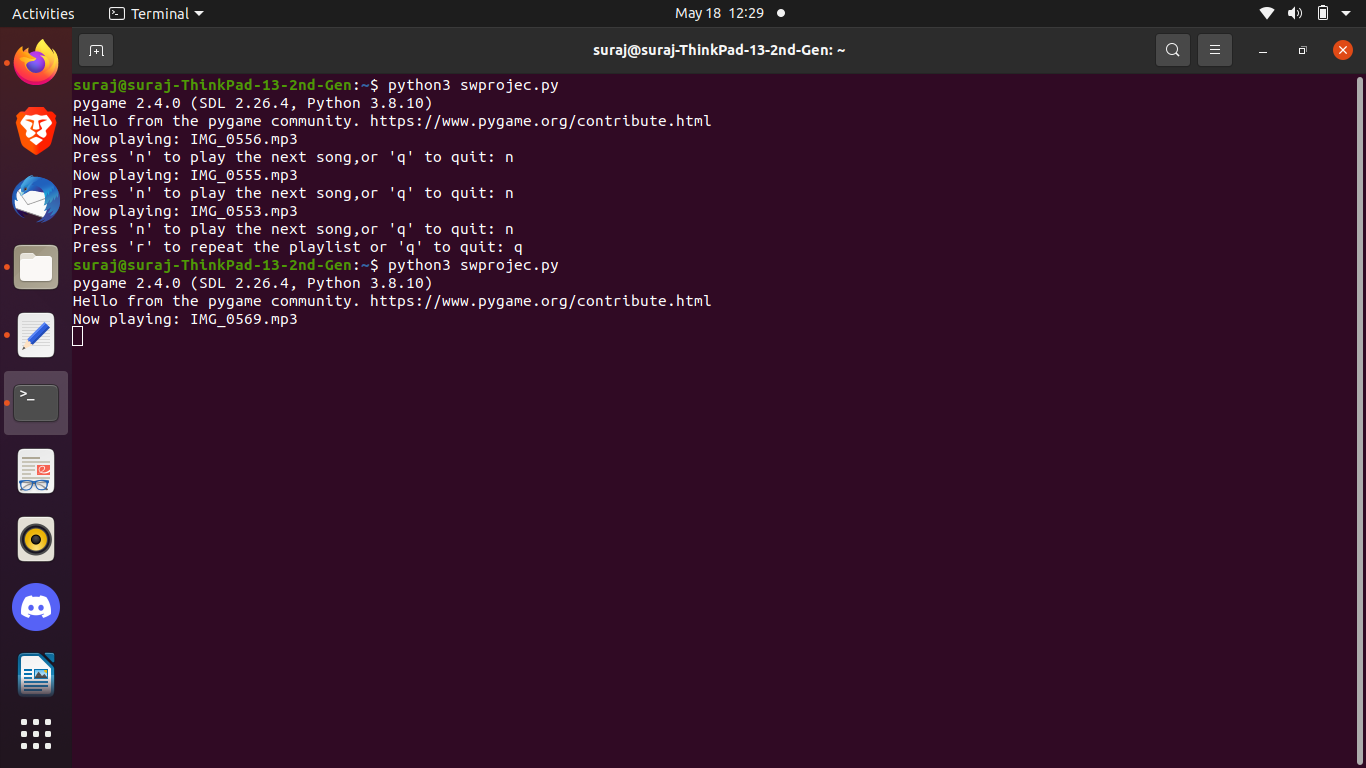
\includegraphics[width = 0.5\textwidth]{figs/fig3.png}
    \caption{Playing songs randomly}
    \label{fig:my_label}
\end{figure}


\subsection{Handling User Input}

During song playback, the program waits until the audio playback is finished using \texttt{pygame.mixer.music.get\_busy()}.
The program prompts the user for input, allowing them to control the playback:
\begin{itemize}
    \item Press 'n' to proceed to the next song.
    \item Press 'q' to exit the playlist, stopping the playback.
\end{itemize}
If the user chooses to proceed to the next song, the program breaks out of the inner while loop and proceeds to the next iteration.

\begin{figure}[h]
    \centering
    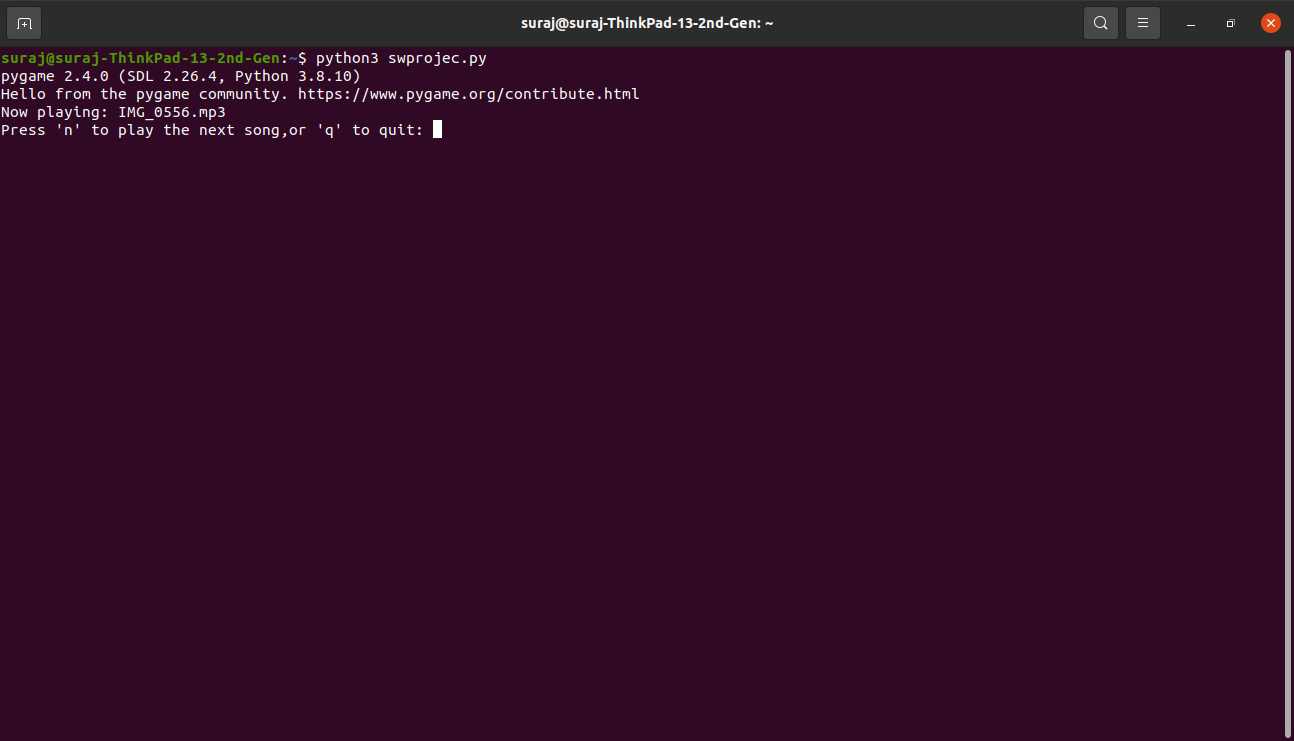
\includegraphics[width = 0.5\textwidth]{figs/fig1.png}
    \caption{Displaying next and quit options}
    \label{fig:my_label}
\end{figure}

\subsection{Repeating or Quitting the Playlist}

After the playlist ends, the program prompts the user to repeat the playlist or quit.
If the user chooses to repeat, the \texttt{play\_random\_playlist()} function is called recursively, restarting the playback with a shuffled playlist.
If the user chooses to quit, the program exits.

\begin{figure}[h]
    \centering
    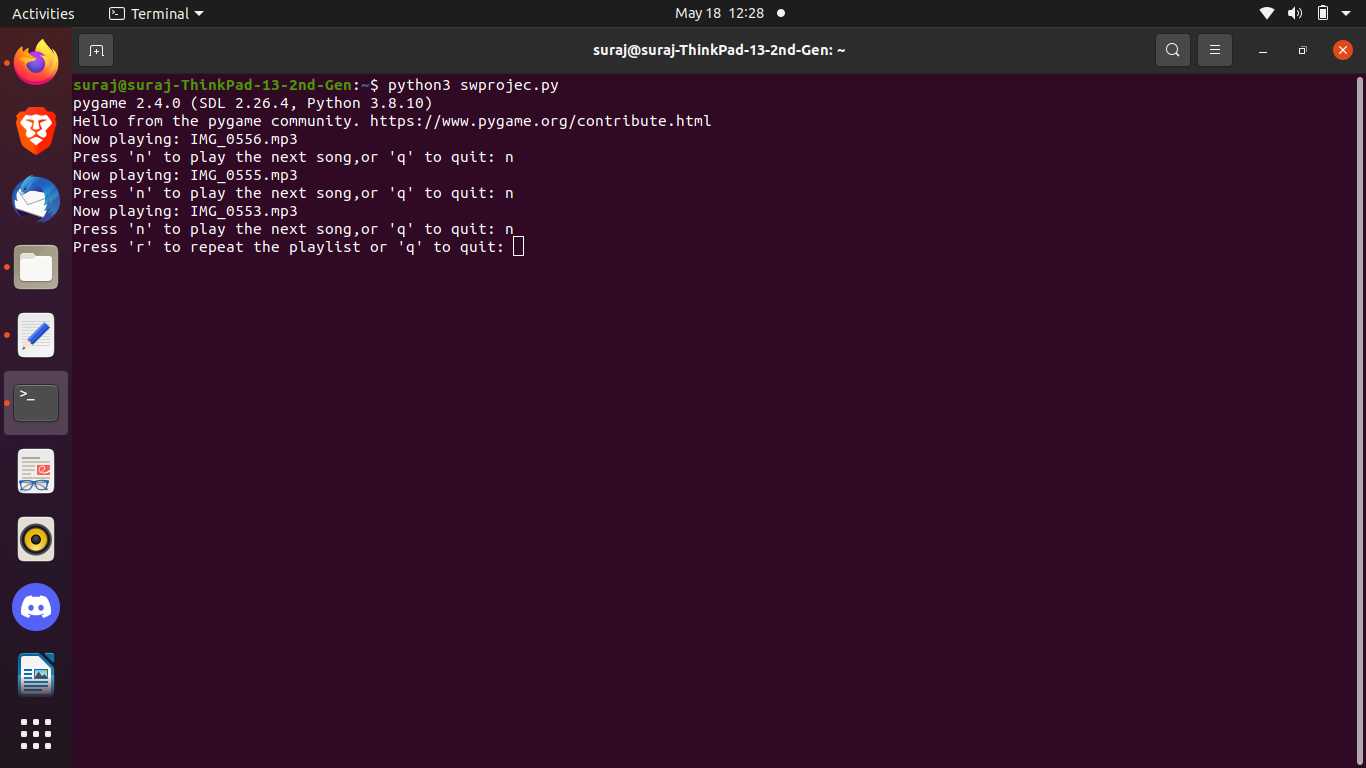
\includegraphics[width = 0.5\textwidth]{figs/fig2.png}
    \caption{Displaying repeat and quit options}
    \label{fig:my_label}
\end{figure}


\section{Results}

The program successfully plays audio files randomly from the specified playlist directory. The songs are shuffled using NumPy, ensuring a random order for each playback. The user can control the playback, skip songs, pause and resume, and exit the playlist as desired.

\section{Conclusion}

The random audio playlist player program provides an interactive and enjoyable experience for users who want to listen to their music playlists in a random order. It utilizes the Pygame library for audio playback, allowing for seamless and efficient handling of audio files. The program's functionality to control the playback, skip songs, pause and resume, and exit the playlist enhances the user experience. Overall, the program fulfills its purpose of playing audio files randomly from a given playlist directory.

\end{document}

